\documentclass[12pt]{article}
\usepackage[OT1]{fontenc}
\usepackage[utf8]{inputenc}
\usepackage{kpfonts}
\usepackage{graphicx}
\usepackage[dvipsnames]{xcolor}
\usepackage{amsthm}
\usepackage[margin=1.25in]{geometry}
\usepackage[sf,bf,small,raggedright,compact]{titlesec}
\usepackage{hyperref}
\definecolor{linkblue}{named}{MidnightBlue}
\hypersetup{colorlinks=true, linkcolor=linkblue,  anchorcolor=linkblue,
        citecolor=linkblue, filecolor=linkblue, menucolor=linkblue,
        urlcolor=linkblue}
\usepackage[capitalize]{cleveref}
\usepackage{paralist}
\usepackage[longnamesfirst,numbers,sort&compress]{natbib}



\newcommand{\pref}[1]{(P\ref{#1})}
\setlength{\parskip}{1ex}

\newtheorem{thm}{Theorem}
\newtheorem{obs}{Observation}
\newtheorem{clm}{Claim}
\newenvironment{clmproof}{\noindent\emph{Proof of Claim:}}{\hfill$\blacksquare$\par}
\newtheorem{lem}{Lemma}

\crefname{dm}{}{}
\creflabelformat{dm}{#2(DM#1)#3}
\crefname{dp}{}{}
\creflabelformat{dp}{#2(DP#1)#3}
\crefname{p}{}{}
\creflabelformat{p}{#2(#1)#3}


\DeclareMathOperator{\dist}{d}
\DeclareMathOperator{\pack}{pack}
\DeclareMathOperator{\hit}{hit}

\newcommand{\defin}[1]{\emph{\textcolor{Maroon}{#1}}}

\newcommand{\pat}[1]{[\textcolor{red}{PM: #1}]}

\title{Connected Dominating Sets in Triangulations}
\author{Prosenjit Bose \and Vida Dujmović \and Hussein Houdrouge \and Pat Morin \and Saeed Odak \and Anyone Else?}
\date{October 2023}



\begin{document}

\maketitle

% \begin{abstract}
%   We show that every $n$ vertex triangulation $G$ has a spanning tree with at least $n/2\pm{?}$ leaves.  This improves the previous best bound of $2n/5\pm {?}$, due to Kleitman and West (1991). \pat{Is this true? I only find $n/3$.}
% \end{abstract}


\section{Introduction}

A set $X$ of vertices in a graph $G$ is a \defin{dominating set} if each vertex of $G$ is in $X$ or adjacent to a vertex in $X$.  A dominating set $X$ of $G$ is \defin{connected} if the induced graph $G[X]$ is connected.

% Observe that, for any connected dominating set $X$, $G$ has a spanning-tree in which all vertices in $V(G)\setminus X$ are leaves.  Similarly, by removing the leaves of any spanning tree of $G$ we obtain a tree whose vertex set is a connected dominating set of $G$.
%  Therefore, an $n$-vertex graph $G$ has a connected dominating set of size $q$ if and only if $G$ has a spanning tree with at least $n-q$ leaves.

The main result in this paper is the following:

\begin{thm}\label{main_result2}
  For any $n\ge 4$, any $n$-vertex triangulation $G$ has a connected dominating set $X$ of size at most $(7n-14)/13$ and there exists an algorithm that finds $X$ in linear time.
\end{thm}

\subsection{Related Work}

Dominating sets in graphs is an enormous field of research, with several books  devoted to the topic \cite{haynes.hedetniemi.ea:domination,haynes.hedetniemi.ea:topics}.

\pat{Expand.  Explain how Kleitman-West result gives $3n/4$.  Explain how Matheson-Tarjan gives $2n/3$.  Talk about connected dominating sets in unit disk graphs.}


% \begin{thm}\label{main_result}
%   For any $n\ge 4$, any $n$-vertex triangulation $G$ has a connected dominating set of size at most $4n/7 + O(1)$.
% \end{thm}


\section{The Proofs}

For a graph $G$, let $|G|=|V(G)|$ denote the number of vertices of $G$.  A \defin{bridge} in a graph $G$ is an edge $e$ of $G$ such that $G-e$ has more connected components than $G$.  For a vertex $v\in G$, $N_G(v):=\{w\in V(G):vw\in E(G)\}$ is the \defin{open neighbourhood} of $v$ in $G$,  $N_G[v]:=N_G(v)\cup\{v\}$ is the \defin{closed neighbourhood} of $v$ in $G$.  For a vertex subset $S\subseteq V(G)$, $N_G[S]:=\bigcup_{v\in S} N_{G}[v]$ is the \defin{closed neighbourhood} of $S$ in $G$ and $N_G(S):=N_G[S]\setminus S$ is the \defin{open neighbourhood} of $S$ in $G$.  A set $X\subseteq V(G)$ \defin{dominates} a set $B\subseteq V(G)$ if $B\subseteq N_G[X]$.  Thus, $X$ is a dominating set of $G$ if and only if $X$ dominates $V(G)$.

A \defin{plane graph} is a graph equipped with a non-crossing embedding in $\mathbb{R}^2$.  A plane graph is \defin{outerplane} if all its vertices appear on the outer face.  A \defin{triangle} is a cycle of length $3$. A \defin{near-triangulation} is a plane graph whose outer face is bounded by a cycle and whose inner faces are all bounded by triangles.  A \defin{generalized near-triangulation} is a plane graph whose inner faces are bounded by triangles.


For a plane graph $H$, we use the notation $B(H)$ to denote the vertex set of the outer face of $H$ and define $I(H):=V(H)\setminus B(H)$.  The vertices in $B(H)$ are \defin{boundary vertices} of $H$ and the vertices in $I(G)$ are \defin{inner vertices} of $H$. For any vertex $v$ of $H$, the \defin{inner neighbourhood} of $v$ in $H$ is defined as $N_H^+(v):=N_H(v)\cap I(H)$, the vertices in $N^+_H(v)$ are \defin{inner neighbours} of $v$ in $H$, and $\deg^+_H(v)=|N^+_H(v)|$ is the \defin{inner degree} of $v$ in $H$.

Let $G$ be a triangulation.  Our procedure for constructing a connected dominating set $X$ begins with an incremental phase that eats away at the triangulation $G$ ``from the outside.'' The process of constructing $X$ is captured by the following definition:   A vertex subset $X\subseteq V(G)$ is \defin{outer-domatic} if it can be partitioned into non-empty subsets $\Delta_0,\Delta_1,\ldots,\Delta_{r-1}$ such that
\begin{compactenum}[(P1)]
    \item $\Delta_0\subseteq B(G)$; \label{outer_face}
    \item $\Delta_i\subseteq B(G-(\bigcup_{j=0}^{i-1}\Delta_j))$ for each $i\in\{1,\ldots,r-1\}$; and \label{incremental}
    \item $G-(\bigcup_{j=0}^{r-1}\Delta_j)$ is outerplanar. \label{outerplanar}
\end{compactenum}

\begin{lem}\label{outer_domatic}
    Let $G$ be a triangulation.  Then any outer-domatic $X\subseteq V(G)$ is a connected dominating set of $G$.
\end{lem}

\begin{proof}
  Suppose $X$ is outer-domatic and let $\Delta_0,\ldots,\Delta_{r-1}$ be the corresponding partition of $X$.  For each $i\in\{1,\ldots,r\}$, let $X_i:=\bigcup_{j=0}^{i-1} \Delta_i$.  First observe that, since $\Delta_0\subseteq B(G)$ is non-empty, $X_i$ contains at least one vertex of $B(G)$, for each $i\in\{1,\ldots,r\}$. We claim that,
  \begin{compactenum}[(P1)]\setcounter{enumi}{3}
    \item for each $i\in\{2,\ldots,r\}$ each vertex in $B(G-X_{i-1})$ is adjacent to some vertex in $X_{i-1}$. \label{adjacent}
  \end{compactenum}
  Indeed, for any $i\in\{2,\ldots,r\}$ and any vertex $v\in B(G-X_{i-1})$ is either in $B(G)$ or adjacent to a vertex in $X_{i-1}$. Even in the former case, (P1) ensures that $v$ is adjacent to a vertex in $X_1=\Delta_0\subseteq X_{i-1}$, because $G[B(G)]$ is a clique.

  We now prove, by induction on $i$, that $G[X_i]$ is connected, for each $i\in\{1,\ldots,r\}$.
  The fact that $G[B(G)]$ is a clique and \pref{outer_face} implies that $G[X_1]=G[\Delta_0]$ is connected. For each $i\in\{2,\ldots,r\}$, the assumption that $G[X_{i-1}]$ is connected, \pref{incremental}, and \pref{adjacent} then imply that $G[X_i]=G[X_{i-1}\cup\Delta_{i-1}]$ is connected.

  In particular $G[X_r]=G[X]$ is connected.  Finally, \pref{adjacent}, with $i=r$ and \pref{outerplanar} implies that $N_G(X_r)=B(G-X_r)=V(G-X_r)$, so $X_r=X$ is a dominating set of $G$.
\end{proof}

We will present two algorithms that grow a connected dominating in small batches $\Delta_0,\Delta_1,\ldots,\Delta_{r-2}$ that result in a sequence of sets $X_1,\ldots,X_{r-1}$ where $X_{i}=\bigcup_{j=0}^{i-1}\Delta_j$.  However, each of these algorithms is unable to continue once they reach a point where each vertex in $B(G-X_i)$ has inner-degree at most $1$ in $G-X_i$.  We begin by studying the graphs that cause this to happen.

\subsection{Critical Graphs}

A generalized near-triangulation $H$ is \defin{critical} if $\deg^+_H(v)\le 1$ for each $v\in B(H)$.


\begin{lem}\label{base_case}
    Let $H$ be a critical generalized near-triangulation. Then $|B(H)|\ge 3|I(H)|$ and there exists $\Delta\subseteq B(H)$ of size at most $|I(H)|$ that dominates $I(H)$.
\end{lem}

\begin{proof}
  Let $B:=B(H)$ and $I:=I(H)$.  If $I$ is empty then the result is trivially true, by taking $X:=\emptyset$, so we now assume that $I$ is non-empty.  By definition, the graph $H[B]$ is outerplanar.  Say that an inner face of $H[B]$ is \defin{marked} if it contains an inner vertex of $H$.  Consider some marked face $f$ of $H[B]$.  This face is marked because it contains at least one vertex in $I$.  Since $H$ is a triangulation, there is an edge $vx$ in $H$ with $v\in B$ on the boundary of $f$ and $x\in I$ in the interior of $f$. Since $G$ is a triangulation and $x$ is an inner vertex of $H$, the edge $vx$ is on the boundary of two faces $vxv_1$ and $vxv_{k-1}$ of $H$ with $v_1\neq v_{k-1}$.  Since $\deg^+_H(v)=1$, each of $v_1$ and $v_{k-1}$ are in $B$.  By the same argument, $H$ contains a face $v_1xv_2$ with $v_2\in B$, $v_2\neq v$, and repeating this argument shows that $v,v_1,v_2,\ldots,v_{k-1}$ is the cycle in $H[B]$ that bounds $f$.  Therefore, $f$ contains exactly one vertex $x_f:=x$ of $I$ and $x_f$ is adjacent to each vertex of $f$.  Thus, $H$ is formed from an outerplanar graph $H[B]$ by adding $|I|$ stars, one in the interior of each marked face of $H[B]$.  Furthermore, since $\deg_H^+(v)=1$ for each $v\in B$, each vertex of $H[B]$ is on the boundary of exactly one marked face.

    \begin{figure}
        \begin{center}
            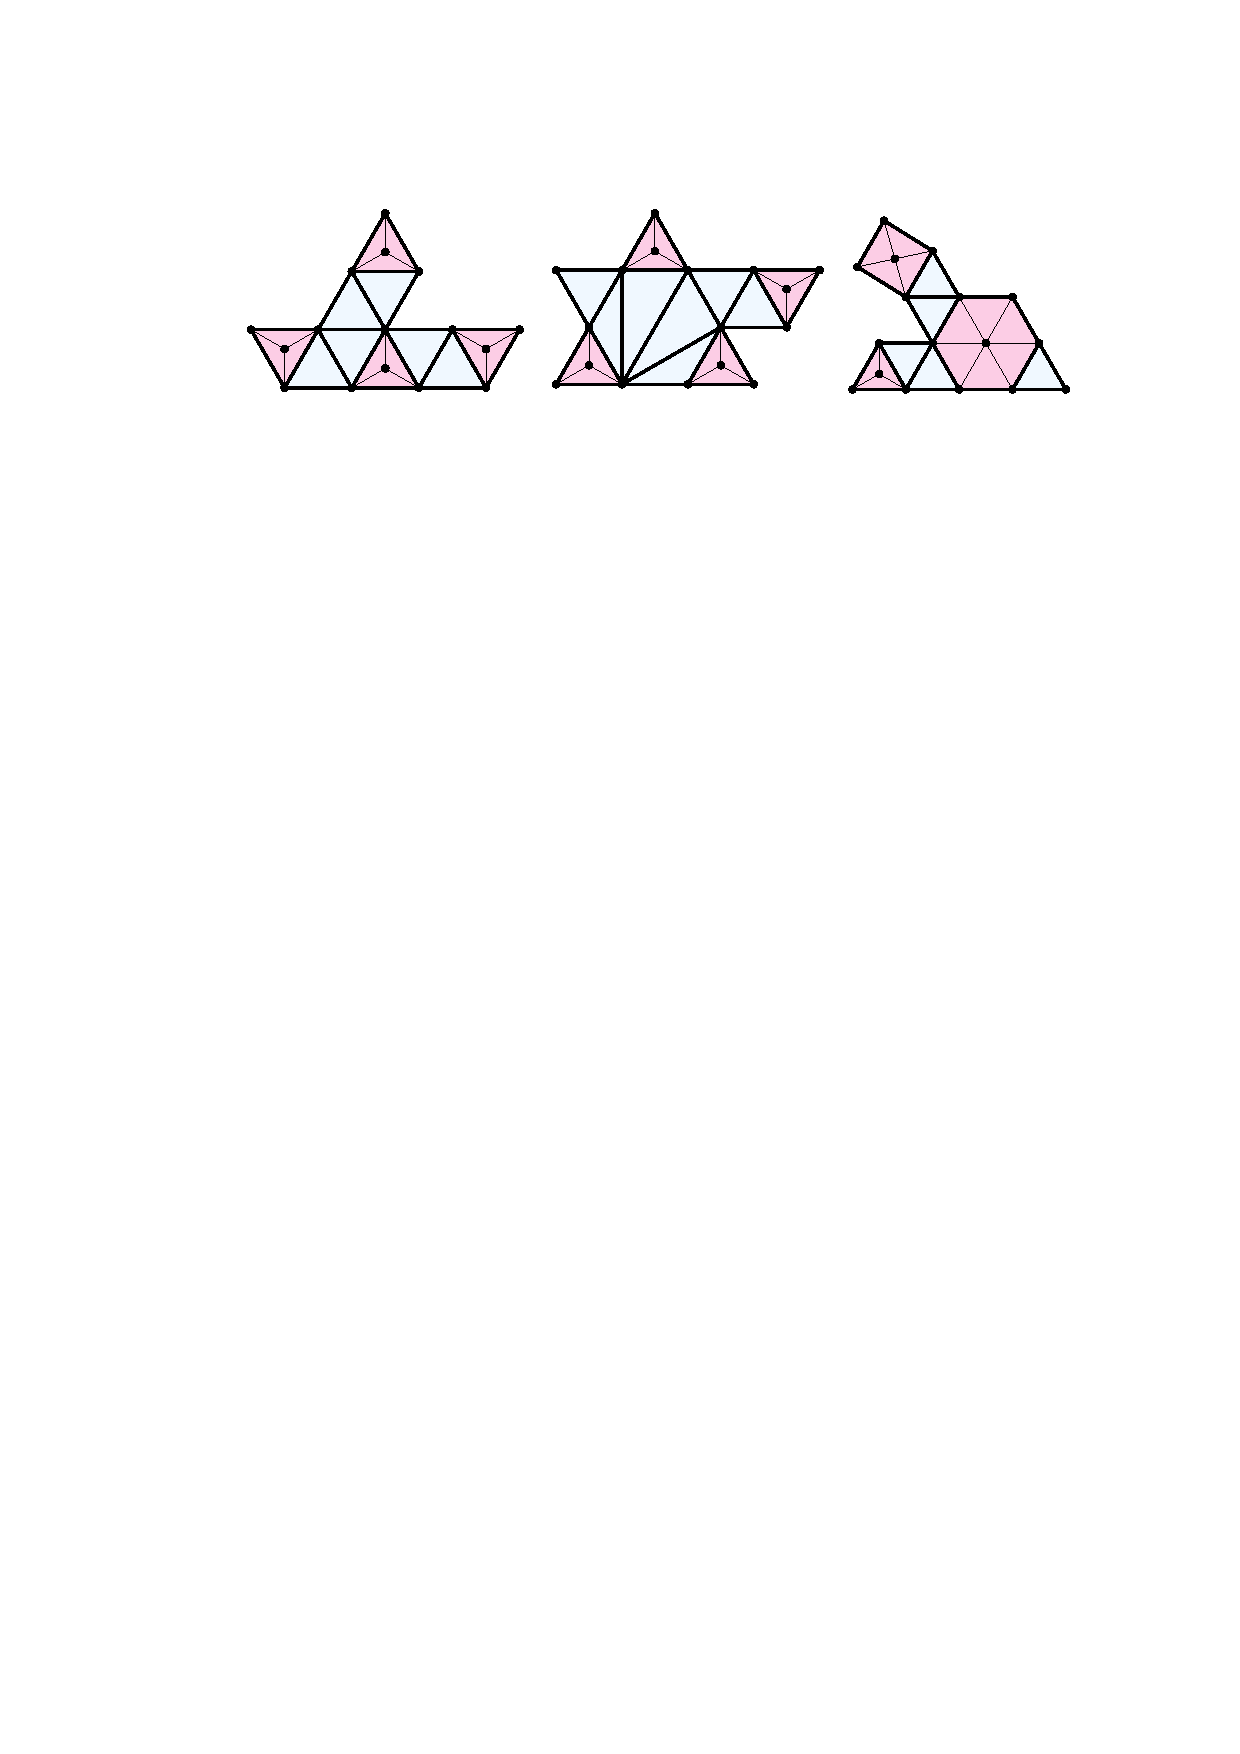
\includegraphics[page=1]{figs/critical} \\
            % \includegraphics[page=2]{figs/critical} \\
        \end{center}
        \caption{Some critical graphs \pat{Add some examples where $H[B(H)]$ has some non-triangular faces}}
        \label{critical_fig}
    \end{figure}

  Consider the graph $H'$ obtained by adding edges to the inner faces of $H[B]$ so that each inner face is a triangle. For each marked face $f$ of $H[B]$, select one triangular face $t_f$ of $H'$ that is contained in $f$ and \defin{mark} $t_f$. Thus there is a bijection from the set of marked faces of $H[B]$ to the set of marked faces in $H'$ and both of these sets have size $|I|$.  Since each vertex in $B$ is on the boundary of at most one marked face of $H[B]$, each vertex in $B$ is on the boundary of at most one marked triangular face of $H'$.  Therefore, $|B| \ge 3|I|$ so $|H|=|B|+|I|\ge 4|I|$. By choosing one vertex from each marked face of $H$ we obtain the desired set $\Delta$.
\end{proof}

\section{A Simple Algorithm}

We start with the simplest possible greedy algorithm, that we call $\textsc{SimpleGreedy}(G)$, to choose $\Delta_0,\ldots,\Delta_{r-1}$.  Suppose we have already chosen $\Delta_0,\ldots,\Delta_{i-1}$ for some $i\ge 0$ and we now want to choose $\Delta_i$.  Let $X_i:=\bigcup_{j=0}^{i-1}\Delta_j$, let $G_i:=G-X_i$, and let $v_i$ be a vertex in $B(G_i)$ that maximizes $\deg^+_{G_i}(v_i)$.  During iteration $i\ge 0$, there are only two cases to consider:
\begin{compactenum}
    \item If $\deg^+_{G_i}(v_i)\ge 2$ then we set $\Delta_i\gets\{v_i\}$.
    \item If $\deg^+_{G_i}(v_i)\le 1$ for all $v\in G_i$ then $G_i$ is critical and this is the final step, so $r:=i+1$.  By \cref{base_case}, there exists $\Delta_i\subseteq B_i$ of size at most $|I_i|$ that dominates $I_i$. Then $X_r:=X_{r-1}\cup\Delta_{i}$ and we are done.
\end{compactenum}

\begin{thm}\label{simple_greedy}
  When applied to an $n$-vertex triangulation $G$,  $\textsc{SimpleGreedy}(G)$ produces a connected dominating set $X_r$ of size at most $(4n-9)/7$.
\end{thm}

\begin{proof}
By the choice of $\Delta_0,\ldots,\Delta_{r-1}$, $X_r$ is an outer-domatic subset of $V(G)$ so, by \cref{outer_domatic}, $X_r$ is a connected dominating set of $G$.  All that remains is to analyze the size of $X_r$.  For each $i\in\{1,\ldots,r\}$, let $D_i:=N_G[X_i]$ be the subset of $V(G)$ that is dominated by $X_i$, let $I_i:=V(G)\setminus D_i$ be the subset of $V(G)$ not dominated by $X_i$, and let $B_i:=N_G(I_i)$ be the vertices of $G$ that have at least one neighbour in each of $X_i$ and $I_i$.  We use the convention that $D_0:=B(G)$.

First observe that, for $i\in\{0,\ldots,r-2\}$, $|D_{i+1}|\ge |D_i|+\deg_{G_i}^+(v_i)$ since $D_{i+1}\supseteq D_i$ and $D_{i+1}$ contains the $\deg_{G_i}^+(v_i)$ inner neighbours of $v_i$ in $G_i$.  Therefore
\[
    |D_{r-1}| \ge |D_0| + \sum_{i=0}^{r-2} \deg_{G_i}^+(v_i) \ge 3 + \sum_{i=0}^{r-2} 2 =  2r+1 \enspace . \label{double_d}
\]
Since $D_{r-1}$ and $I_{r-1}$ partition $V(G)$,
\begin{equation}
  n = |D_{r-1}| + |I_{r-1}| \ge 2r+1 + |I_{r-1}|  \enspace . \label{c1}
\end{equation}
% so
% \begin{equation}
%     r\le \frac{n-|I_{r-1}|-1}{2}  \enspace .
% \end{equation}

Since $X_{r-1}$ and $B_{r-1}$ are disjoint and $D_{r-1}\supseteq B_{r-1}\cup X_{r-1}$, we have $|D_{r-1}|\ge |X_{r-1}| + |B_{r-1}|=r-1+|B_{r-1}|$.  Therefore,
\begin{align}
    n & = |D_{r-1}| + |I_{r-1}| \ge r-1 + |B_{r-1}| + |I_{r-1}| = r-1 + |B_{r-1}| + |I_{r-1}| \notag
    \\
    & \ge r - 1 + 4|I_{r-1}| \enspace , \label{c2}
\end{align}
where the last inequality follows from \cref{base_case}.

The final dominating set $X_r$ has size $|X_r| = |X_{r-1}| + \Delta_{r-1} = r - 1 +|I_{r-1}|$, so the size of $|X_r|$ can be upper-bounded by maximizing $r-1+|I_{r-1}|$ subject to \cref{c1,c2}.  More precisely, by setting $x:=r$ and $y:=|I_{r-1}|$, the maximum size of $X_r$ is upper-bounded by the maximum value of $x-1+y$ subject to the constraints
\begin{align*}
  x - 1 + 4y & \le n \\
  2x + 1 + y & \le n
\end{align*}

% r\le (n+1-I_{r-1})/2$ and $r+4|I_{r-1}|\le n$.
This is an easy linear programming exercise and the maximum value of $X_{r}$ is obtained when $r=(3n-5)/7$ and $|I_{r-1}|=(n+3)/7$, which gives
$|X_r| \le (4n-9)/7$.
\end{proof}


We note that the implementation of $\textsc{SimpleGreedy}(G)$ is even simpler than the definition given above.  Nothing special needs to be done for the critical graph $G_{r-1}$.  Repeatedly selecting a vertex of maximum innner-degree and removing it will produce a dominating set of size exactly $|I_{r-1}|$.  Thus, $\textsc{SimpleGreedy}(G)$ has a simple linear time implementation.  In this implementation, each vertex $v$ stores a value $d_v$ which is initially set to $\deg_G(v)$.  For the three vertices on the outer face of $G$, $d_v$ is initially set to $\deg_G(v)-2$.  In general, $d_v$ is kept updated so that it is always equal to the inner-degree of $v$ in $G_i$.

Besides the data structure used for representing the triangulation $G$, each vertex $v$ also participates in a doubly-linked list $L_{d_v}$  that stores all the vertices with the same $d_v$ value.  A global doubly-linked list $L$ then stores all the lists $L_d$ such that $L_d$ is non-empty, sorted by increasing order of $d$.   Extracting a vertex of maximum inner-degree can then be done in constant time and the total time spent moving vertices between different lists in $L$ is proportional to the number of edges of $G$. Thus, the entire algorithm can be implemented in $O(n)$ time.

\section{A Less Simple Algorithm}

Next we devise an algorithm that produces a smaller connected dominating set than what is guaranteed by $\textsc{SimpleGreedy}(G)$.  This involves a more careful analysis of the cases in which \textsc{SimpleGreedy} is forced to take a vertex $v_i$ with $\deg^+_{G_i}(v_i)=2$.  We begin by identifying unnecessary vertices and edges that can appear in the graphs $G_1,\ldots,G_{r-1}$ during the construction of $X$.   We say that a near-triangulation $H$ is \defin{dom-minimal} if
\begin{compactenum}[({DM}1)]
    \item each vertex $v\in B(H)$ has $\deg^+_H(v)\ge 1$; and \label{bad_vertex}
    \item each edge $vw$ on the boundary of the outer face of $H$ is on the boundary an inner face $vwx$ of $H$ for some $x\in I(H)$. \label{bad_edge}
\end{compactenum}
We say that a generalized near-triangulation $H$ is \defin{dom-minimal} if each of its biconnected components are dom-minimal.

\begin{obs}\label{bridgeless}
    Any dom-minimal generalized near-triangulation $H$ is bridgeless.
\end{obs}

\begin{proof}
   If $vw$ is a bridge in $H$ then both $v$ and $w$ are in $B(H)$.  Since $vw$ is a bridge in $H$, there is no inner face $vwx$ in $H$. Thus $H$ does not satisfy the second condition for dom-minimality.
\end{proof}

A subgraph $H'$ of a generalized near-triangulation $H$ is \defin{dom-preserving} if
\begin{compactenum}[({DP}1)]
  \item $B(H')\subseteq B(H)$;
  \item $N^+_{H'}(v)=N^+_H(v)$ for all $v\in B(H')$;
  \item $I(H')=I(H)$; and
  \item $N_{H'}(v)=N_H(v)$ for all $v\in I(H)$.
\end{compactenum}

\begin{obs}
  Let $H$ be a generalized near-triangulation, let $H'$ be a dom-preserving subgraph of $H$, and let $\Delta$ be a subset of $V(H)$ that dominates $I(H)$.  Then $\Delta\cap V(H')$ dominates $I(H)$.
\end{obs}

\begin{proof}
  Each vertex $v\in I(H')$ is adjacent to some vertex $w\in \Delta$.  Since $N_{H'}(v)=N_H(v)$, $w\in\Delta\cap V(H')$, so $v$ is dominated by $\Delta\cap V(H')$.  Since this is true for each $v\in I(H)=I(H')$, $\Delta\cap V(H')$ dominates $I(H)$.
\end{proof}

\begin{lem}\label{dom_minimal}
  For any generalized near-triangulation $H$, there exists a dom-preserving subgraph $H'$ of $H$ that is dom-minimal.
\end{lem}

\begin{proof}
  The proof is by induction on $|V(H)|+|E(H)|$.  If $H$ is already dom-minimal, then setting $H'=H$ satisfies the requirements of the lemma, so assume that $H$ is not dom-minimal.  It is straightforward to verify that the dom-preserving subgraph relationship is transitive, so if $H$ has a dom-preserving subgraph $H^*$ and $H^*$ has a dom-preserving subgraph $H'$ then $H'$ is a dom-preserving subgraph of $H$.  Therefore, it is sufficient to show the existence of a dom-preserving subgraph $H^*$ of $H$ with fewer edges or fewer vertices than $H$, and the inductive hypothesis provides the desired dom-minimal dom-preserving subgraph $H'$ of $H$.

  If $H$ contains a vertex $v\in B(H)$ with $\deg^+_H(v)=0$ then $H-v$ is a dom-preserving subgraph of $H$ with fewer vertices than $H$.  We now assume that $\deg^+_H(v)\ge 1$ for all $v\in B(H)$.  Since $H$ is not dom-minimal then $H$ contains a biconnected component $C$ that is not dom-minimal.
  \begin{compactenum}
    \item If there exists an edge $vw$ on the outer face of $C$ that is not incident to any inner face $vwx$ with $x\in I(C)$ then $B(H-vw)=B(H)$ and $I(H-vw)=I(H)$, and $H-vw$ is a is dom-preserving subgraph of $H$ that has fewer edges than $H$.

    \item If there exists a vertex $v\in B(C)$ with $\deg^+_C(v)=0$ then $v$ is incident to an edge $vw$ that is on the outer face of $C$ and on the outer face of $H$. Since $\deg^+_C(v)=0$, $vw$ is not incident to any inner face $vwx$ with $x\in I(C)$ and we can proceed as in the previous case. \qedhere
  \end{compactenum}
\end{proof}

% We say that a generalized near-triangulation $H$ is \defin{good} if
% \begin{compactenum}[(G1)]
%       \item $H$ is critical;
%       \item there exists $v\in B(H)$ with $\deg^+_H(v)\ge 3$; or
%       \item there exists distinct $v,w\in B(H)$ such that $\deg^+_H(v)=2$ and $N^+_H(w)\subseteq N^+_H(v)$.
% \end{compactenum}
%
% \begin{lem}\label{not_good}
%   Let $H$ be a dom-minimal generalized near-triangulation.  Then \begin{compactenum}[(i)]
%     \item $H$ is good or
%     \item $B(H)$ contains a vertex $v$ with $\deg^+_H(v)=2$ such that $G-v$ is good.
%   \end{compactenum}
% \end{lem}
%
% \begin{proof}
%   Since $H$ is dom-minimal, each vertex in $B(H)$ has inner-degree greater than $0$.  If some vertex in $B(H)$ has inner-degree at least $3$ then $H$ is good and there is nothing to prove, so we may assume that each vertex in $B(H)$ has inner-degree $1$ or $2$.  Since $H$ is not critical, at least one vertex in $B(H)$ has inner-degree $2$.  We distinguish between two cases, depending on whether $H$ is biconnected.
%
%   \pat{Updated here. The case where $H$ is biconnected needs a separate argument when $k=3$.}
%   If $H$ is biconnected then, since $H$ is bridgeless (by \cref{bridgeless}) the outer face of $C$ is a cycle $v_0,\ldots,v_{k-1}$ with $k\ge 3$. If there exists an edge $v_iv_{i+1}$ of this cycle with $\deg^+_H(v_i)=2$ and $\deg^+_H(v_{i+1})=1$ then $N_H^+(v_{i+1})\subset N_H^+(v_i)$ and $H$ is good, so we may assume that $\deg^+_H(v_i)=2$ for all $i\in\{0,\ldots,k-1\}$.
%   Let $v_i$ be a vertex in $B(H)$ such that $N_H(v_i)=N_H^+(v_i)\cup\{v_{i-1},v_{i+1}\}$.  Without loss of generality, assume $i=0$. Now consider the graph $H'=H-v_0$.  This graph contains two vertices, namely $v_{1}$ and $v_{k-1}$ with inner-degree $1$.  If $k\ge 4$, then $H'$ is good, because $\deg_{H'}^+(v_2)=2$ and $N^+_{H'}(v_1)\subseteq N^+_{H'}(v_2)$.  Otherwise, the outer face of $H'$ is a $4$-cycle $x_1,x_2,v_1,v_2$ and $N_H^+(v_1)\subseteq N_H^+(x_2)$ and $N_H^+(v_2)\subseteq N_H^+(x_1)$.  If $\deg^+_H(x_2)\ge 2$ or $\deg^+_H(x_1)\ge 2$ then $H'$ is good.  Otherwise all vertices in $B(H')$ have inner-degree at most $1$ in $H'$, so $H'$ is also good. Therefore $H$ contains a vertex $v:=v_0$ such that $H-v$ is good, as required.
%
%
%
%   If $H$ is not biconnected, then let $C$ be a biconnected component of $H$ that contains a single cut-vertex $v_0$ of $H$ (so $C$ is a leaf in the block-cut tree of $H$). Then $v_0$ is contained in a second biconnected component $C'\neq C$ of $H$. Since $H$ is dom-minimal, $\deg^+_{C}(v_0)\ge 1$ and $\deg^+_{C'}(v_0)\ge 1$, so $\deg^+_H(v)= 2$.
%
%   Since $C$ is biconnected, its outer face is bounded by a cycle $v_0,v_1,v_2,\ldots,v_{k-1}$.  If $\deg^+_C(v_1)=1$ then, since $H$ is dom-minimal, the edge $v_0v_1$ is on the boundary of an inner face $v_0v_1x$ with $x\in I(H)$.  Since $v_0$ is the only cut-vertex of $H$ in $C$, $N^+_H(v_1)=N^+_C(v_1)=\{x\}\subseteq N_H(v_0)$ and $\deg^+_H(v_0)=2$, so $H$ is good and there is nothing to prove.  We may therefore  assume that $\deg^+_C(v_1)=2$ and,  by the same reasoning, that $\deg^+_C(v_i)=2$ for each $i\in\{1,\ldots,k-1\}$.  (Otherwise, $N^+_H(v_i)\subseteq N^+_H(v_{i-1})$ and $\deg^+_H(v_{i-1})=2$ for some $i\in\{2,\ldots,k-1\}$ so $H$ is good.)
%
%   To summarize, so far we know that some vertex $x\in I(H)$ is in $N^+_H(v_0)$, $N^+_H(v_1)$, and $N^+_H(v_{k-1})$.  If $k=3$ then, since $H$ is dom-minimal, $H$ contains a face $v_1v_{k-1}y$ with $y\in I(H)$.  Since $\deg^+_H(v_1)=\deg^+_H(v_{k-1})=2$, $y\neq x$ and $N^+_H(v_1)=N^+_H(v_2)=\{x,y\}$. Again, this implies that $H$ is good.  We now assume that $k\ge 4$.
%
%   The edge $v_1v_2$ is on the boundary of a face $v_1v_2y$.  Since $\deg^+_H(v_1)=2$, $x\neq y$.  If $N^+_H(v_1)=N^+_H(v_2)=\{x,y\}$ then $v_1$ and $v_2$ satisfy (GM3), so $H$ is good.  Otherwise, consider the graph $H':=H-v_0$.  Then $\deg^+_{H'}(v_1)=1$, $\deg^+_{H'}(v_2)=2$, and $N_{H'}(v_1)\subseteq N_{H'}(v_2)$.   Therefore $H'$ is good, so $H$ contains a vertex $v=v_0$ of inner-degree $2$ such that $H-v$ is good.  This completes the proof.
% \end{proof}
%
%
% This gives variant of the $\textsc{SimpleGreedy}(G)$ that we call $\textsc{BetterGreedy}(G)$.  Suppose we have already chosen $\Delta_0,\ldots,\Delta_{i-1}$ for some $i\ge 0$ and we now want to choose $\Delta_i$.  Let $X_i:=\bigcup_{j=0}^{i-1}\Delta_j$, let $G_i$ be a dom-preserving subgraph of $G-X_i$ that is dom-minimal, and let $v_i$ be a vertex in $B(G_i)$ that maximizes $\deg^+_{G_i}(v_i)$.  During iteration $i\ge 0$, there are now four cases to consider:
% \begin{compactenum}
%     \item If $\deg^+_{G_i}(v_i)\ge 3$ then we set $\Delta_i\gets\{v_i\}$.
%     \item If there exists distinct $v_i,w\in B(H)$ such that $\deg^+_H(v_i)=2$ and $N^+_H(w)\subseteq N^+_H(v_i)$ then set $\Delta_i:=\{v_i\}$.
%     \item If $\deg^+_{G_i}(v_i)\le 1$ for all $v\in G_i$ then $G_i$ is critical and this is the final step, so $r:=i+1$.  By \cref{base_case}, there exists $\Delta_i\subseteq B_i$ of size at most $|I_i|$ that dominates $I_i$. Then $X_r:=X_{r-1}+\Delta_{i}$ and we are done.
%     \item Otherwise, $G_i$ is not good.  By \cref{not_good}, $G$ contains a vertex $v_i$ of inner-degree $2$ such that $G-v_i$ is good.  Set $\Delta_i:=\{v_i\}$.
% \end{compactenum}
%
% \begin{thm}\label{better_greedy}
%   When applied to an $n$-vertex triangulation $G$,  $\textsc{BetterGreedy}(G)$ produces a connected dominating set $X_r$ of size at most $(7n-14)/13$.
% \end{thm}
%
% \begin{proof}
%   Let $x_2$ be the number of times $\textsc{BetterGreedy}(G)$ falls into Case~4.
%   For each integer $t\ge 3$, let $x_t$ be the number of times $\textsc{BetterGreedy}(G)$ falls into case $1$ and chooses $v_i$ such that $\deg^+_{G_i}(v_i)=t$.  Let $z$ be the number of times $\textsc{BetterGreedy}(G)$ falls into Case~2.  From \cref{not_good}, we know that Case~4 never occurs during two consecutive iterations.  Therefore,
%   \begin{equation}
%       x_2 \le \sum_{t\ge 3}x_t + z + 1 \enspace .  \label{a1}
%   \end{equation}
%   The size of the dominated set $D_{r-1}$ is at least $|D_{r-1}| \ge 3 + \sum_{t\ge 2}tx_t + 2z$.
%   Since $|D_{r-1}|+|I_{r-1}|=n$,
%   \begin{equation}
%    3 + \sum_{t\ge 2}tx_t + 2z + I_{r-1} \le |D_{r-1}| + I_{r-1} \le n  \enspace . \label{a2}
%   \end{equation}
%   The of the boundary $B_{r-1}$ is at most $|B_{r-1}|\le 3+\sum_{t\ge 2}(t-1)x_t$.
%   By \cref{base_case},
%   \begin{equation}
%     3+\sum_{t\ge 2}(t-1)x_t \ge |B_{r-1}| \ge 3|I_{r-1}| \label{a3}
%   \end{equation}
%   The size of the final set $X_{r}$ is
%   \begin{equation}
%     |X_r| = \sum_{t\ge 2}x_t + z + |I_{r-1}| \enspace . \label{objective2}
%   \end{equation}
%   The unbounded number of variables $x_t$, $t\ge 2$ is problematic. We resolve this with the following claim:
%   \begin{clm}
%     In any assignment of non-negative values to $|I_{r-1}|$, $z$, and $x_2,x_3,\ldots$ that maximizes \cref{objective2} subject to \cref{a1,a2,a3}, $x_t=0$ for each $t\ge 3$.
%   \end{clm}
%   \begin{clmproof}
%      If $x_t = c >0$ for some $t\ge 3$, then we can set $x_t\gets 0$, $z\gets z+tc/2$, and $|I_{r-1}|\gets |I_{r-1}|-(t-1)c/3$.  This increases the value of \cref{objective2} by $tc/2-(t-1)c/3 =(t+2)c/6>0$.  The new values still satisfy \cref{a1} because the right hand side of \cref{a1} increases and the left hand side is unchanged.  The new values still satisfy \cref{a2} because the left hand side of \cref{a2} changes by $tc - 2tc/2 = 0$.  The new values still satisfy \cref{a3} because the left and right hand sides of \cref{a3} each decrease by $(t-1)c$.
%   \end{clmproof}
%   Therefore, \cref{a1,a2,a3} are three inequalities in three non-negative variables $x_2$, $z$, and $|I_{r-1}|$.  Maximizing \cref{objective2} subject to these constraints is an easy linear programming exercise that gives $x_2:=(3n-6)/13$, $z=(3n-19)/13$ and $I_{r-1}=(n+11)/13$, which gives $|X_r|= (7n+8)/13$.
% \end{proof}
%

% \section{The Best Algorithm}
% Let's see if we can beat $\textsc{BetterGreedy}(G)$.
% First, we need to rework our definition of dom-minimal a little bit:
%
% We say that a near-triangulation $H$ is \defin{dom-minimal} if
% \begin{compactenum}[({DM}1)]
%     \item there are no two vertices $v,w\in B(H)$ such that $N^+_H(w)\subseteq N^+_H(v)$; and
%     \item each edge $vw$ on the boundary of the outer face of $H$ is on the boundary of an inner face $vwx$ of $H$ for some $x\in I(H)$.
% \end{compactenum}
% We say that a generalized near-triangulation $H$ is \defin{dom-minimal} if each of its biconnected components are dom-minimal.
% Note that (DM1) implies that, unless $|H|=1$, each vertex $v\in B(H)$ has $\deg^+_H(v)\ge 1$.
%
% \Cref{bridgeless,dom_minimal} still hold under this new definition of dom-minimal.
%
% \pat{Did I really need to change the definition of dom-minimal?  Check.}

\begin{lem}\label{chord_incident}
  let $H$ be a dom-minimal near-triangulation and let $v_0$ be a vertex in $B(H)$ with $|N_H(v_0)\cap B(H)|\ge 3$.  Then $\deg^+_H(v_0)\ge 2$.  In other words, if $v_0$ is incident to a chord of the outerplane graph $H[B(H)]$, then $v_0$ is incident to at least $2$ inner vertices of $H$.
\end{lem}

\begin{figure}[htbp]
  \begin{center}
    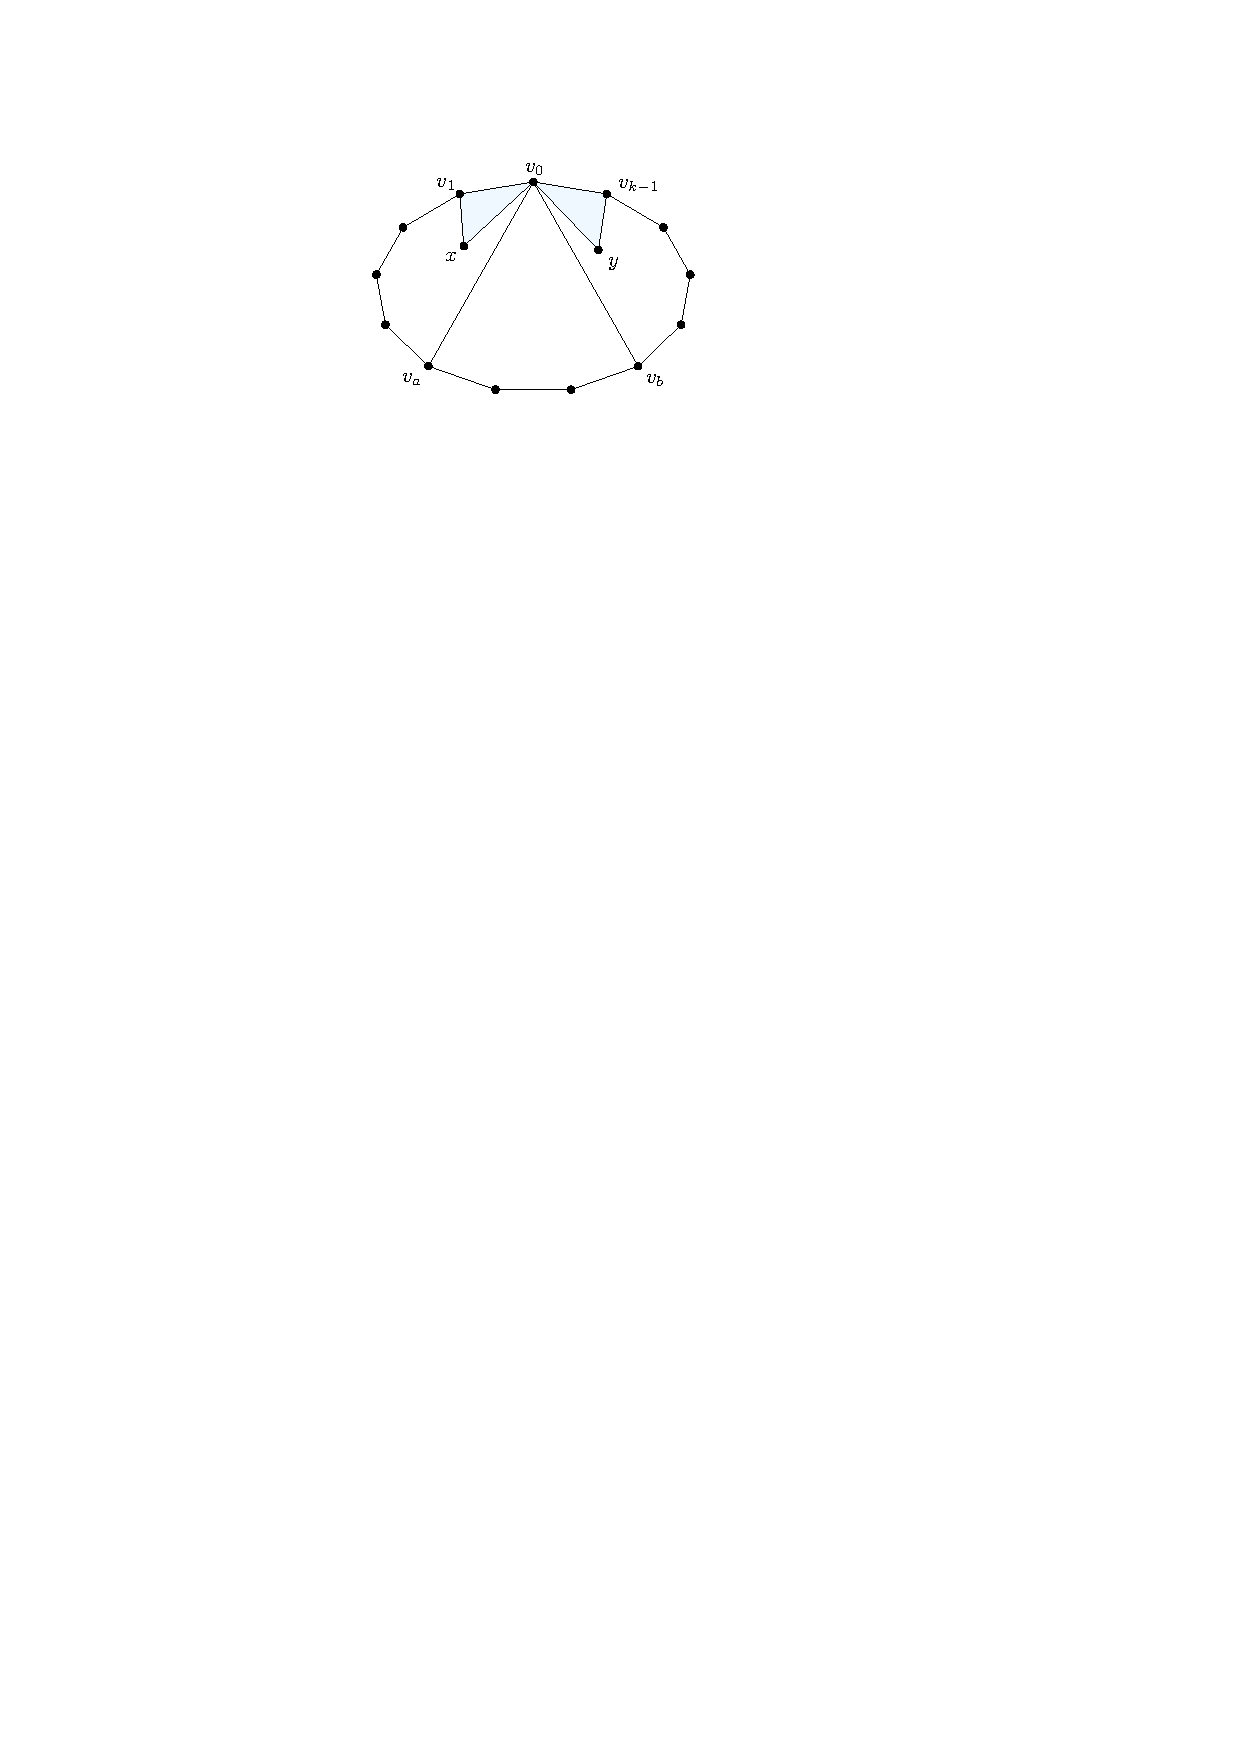
\includegraphics{figs/chord_incident}
  \end{center}
  \caption{The proof of \cref{chord_incident}}
  \label{chord_incident_fig}
\end{figure}
\begin{proof}
  Refer to \cref{chord_incident_fig}
  Since $H$ is a near-triangulation its outer face is bounded by a cycle $v_0,\ldots,v_{k-1}$.  Let $a:=\min\{i\in\{2,\ldots,k-2\}:v_0v_i\in E(H)\}$ and $b:=\max\{i\in\{2,\ldots,k-2\}:v_0v_i\in E(H)\}$. (Possibly $a=b$, but both $a$ and $b$ are well-defined since $|N^+_H(v_0)|\ge 3$.)   Since $H$ is dom-minimal, the edge $v_0v_1$ is on the boundary of an inner face $v_0v_1x$ of $H$ where $x$ is an inner vertex of $H$.  Since $H$ is dom-minimal, the edge $v_{k-1}v_0$ is on the boundary of an inner face $v_{k-1}v_0y$ of $H$ where $y$ is an inner vertex of $H$.  Then $x$ is in the interior of the face of $H[B(H)]$ bounded by the cycle $v_0,v_1,\ldots,v_a$ and $y$ is in the interior of the face of $H[B(H)]$ bounded by the cycle $v_0,v_b,\ldots,v_{k-1}$.  Therefore, $x\neq y$ and $N^+_H(v_0)\supseteq\{x,y\}$ so $\deg^+_H(v_0)\ge 2$.
\end{proof}

\begin{lem}\label{degree_2_outer_neighbour}
  Let $H$ be a dom-minimal near-triangulation. Then either:
  \begin{compactenum}
    \item $H$ is outerplane;
    \item $H$ consists of a cycle on the vertices in $B(H)$ plus one dominant inner vertex $w$; or
    \item each vertex $w\in B(H-B(H))$ has a neighbour $v$ in $H$ with $\deg^+_H(v)\ge 2$.
  \end{compactenum}
\end{lem}

\begin{proof}
   If $H$ is outerplane then there is nothing to prove, so assume otherwise. Let $w$ be a vertex in $B(H-B(H))$. Since $w\not\in B(H)$, $w$ is an inner vertex of $H$. Consider the face $f:=v_0,\ldots,v_{k-1}$ of the outerplane graph $H[B(H)]$ that contains $w$. See \cref{degree_2_outer_neighbour_fig}.

   \begin{figure}[htbp]
     \begin{center}
       \begin{tabular}{cc}
         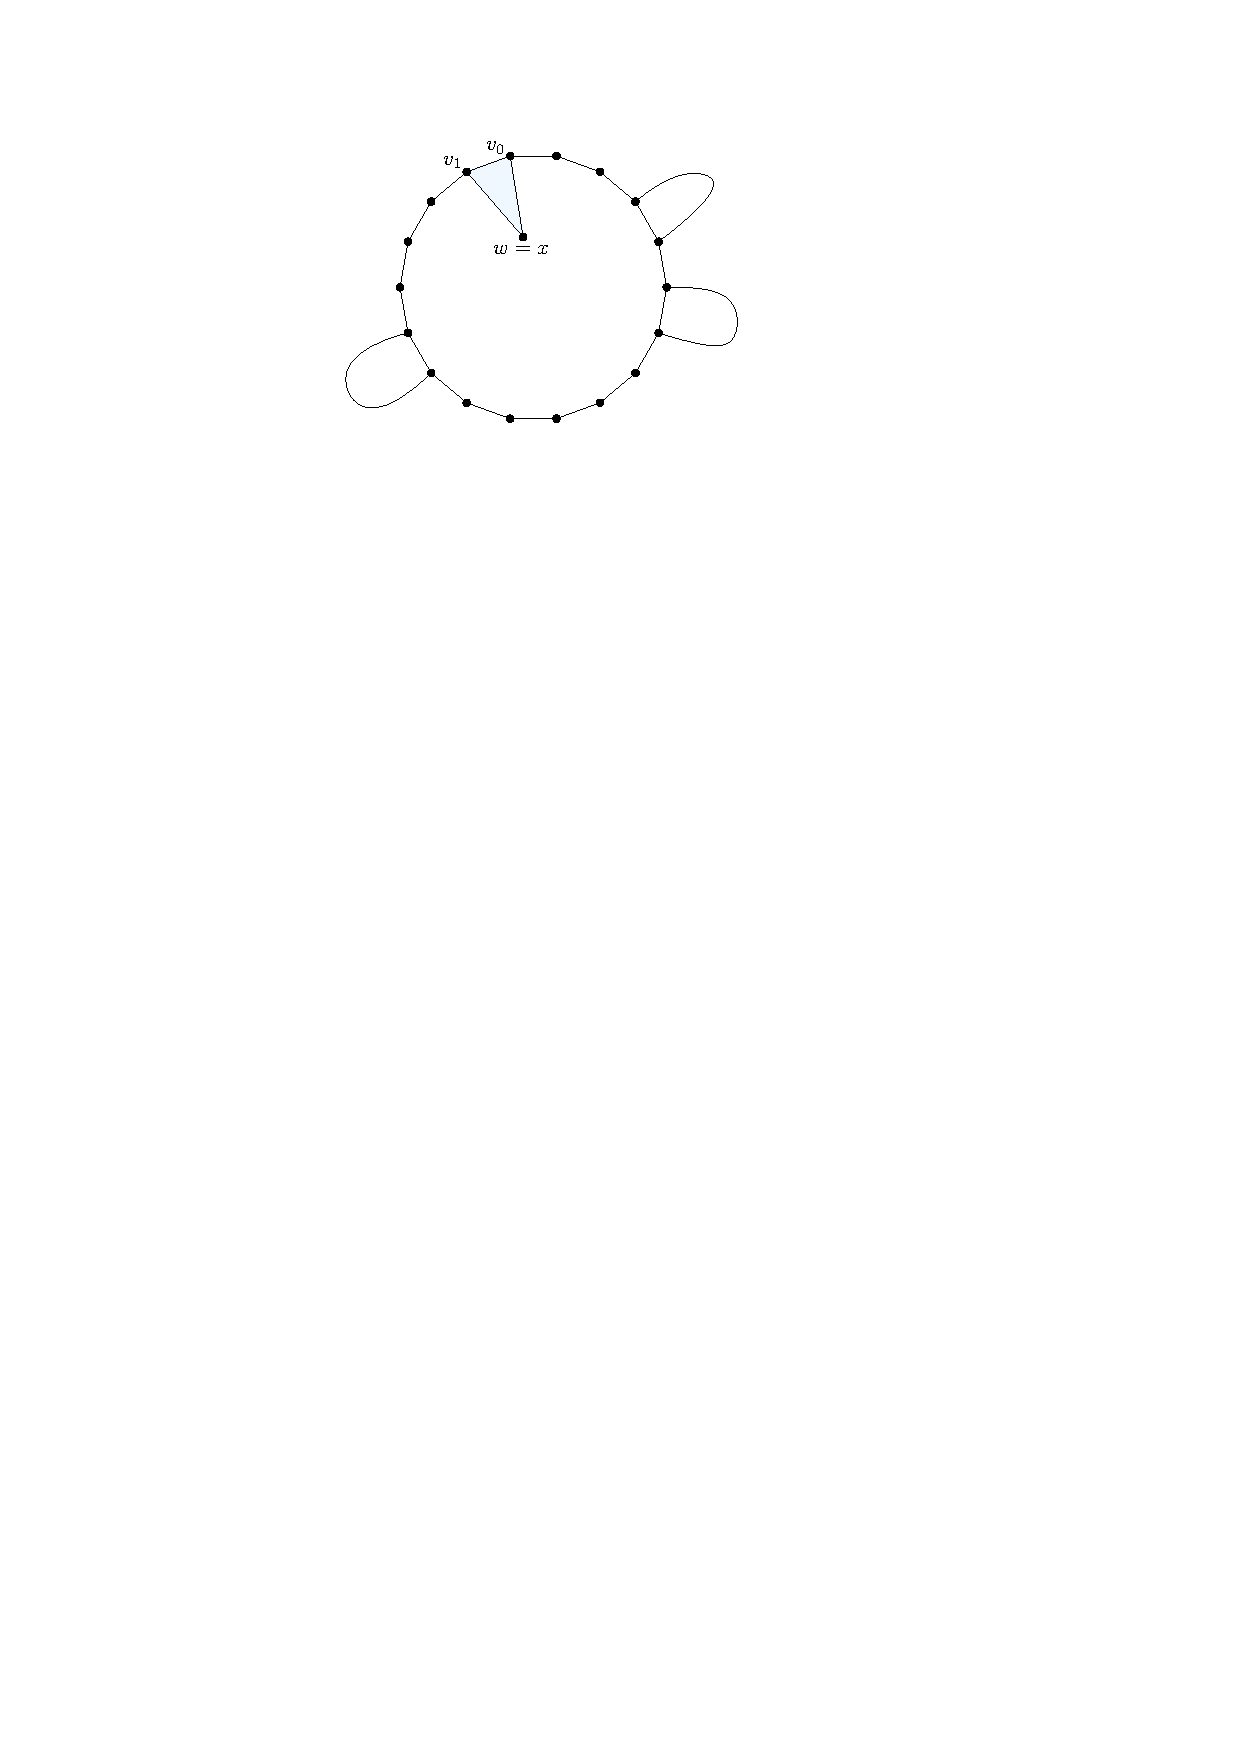
\includegraphics[page=1]{figs/degree_2_outer_neighbour} &
         \includegraphics[page=2]{figs/degree_2_outer_neighbour}
       \end{tabular}
     \end{center}
     \caption{The proof of \cref{degree_2_outer_neighbour}.}
     \label{degree_2_outer_neighbour_fig}
   \end{figure}

   Since $w\in B(H-B(H))$, $w$ is adjacent to at least one vertex, say $v_0$, of $f$.  If $v_0v_{1}$ is a chord of $H[B(H)]$ then, by \cref{chord_incident}, $\deg^+_H(v_0)\ge 2$ and we are done, so assume that $v_0v_{1}$ is not a chord of $H[B(H)]$.  Since $H$ is dom-minimal, $H$ contains an inner face $v_0v_{1}x$ where $x$ is an inner vertex of $H$.  If $x\neq w$, then $\deg_H^+(v_0)\ge 2$ and we are done, so assume that $x=w$.  Therefore, $w$ is adjacent to $v_1$.  Thus, by assuming that $\deg^+_H(v_0)\le 2$ and that $v_0w$ is an edge of $H$ we were able to show that $v_0v_1$ is not a chord of $H[B(H)]$ and that $v_0v_1w$ is an inner face of $H$. This latter fact implies that $v_1w$ is an edge of $H$, so we can repeat this argument to establish that $\deg^+_H(v_j)\ge 2$ for some $j\in\{0,\ldots,k-1\}$ or that $v_{j}v_{j+1}$ is not a chord of $H[B(H)]$ and that $v_{j}v_{j+1}w$ is an inner face of $H$ for all $j\in\{0,\ldots,k-1\}$.  In the first case we are obviously done. In the latter case, $H$ is the graph described in the second alternative given by the lemma.
\end{proof}

\begin{lem}\label{really_good}
  Let $H$ be a dom-minimal generalized near-triangulation.  Then either:
  \begin{compactenum}[(1)]
    \item $H-B(H)$ is critical; \label[p]{two_critical}
    \item $B(H)$ contains a vertex $v$ with $\deg^+_H(v)\ge 3$; or \label[p]{degree_three}
    \item $H$ contains distinct vertices $v_0$, $v_j$, and $w$ such that
    \begin{compactenum}[(a)]
      \item $v_0\in B(H)$ and $\deg^+_H(v_0)=2$;
      \item $w\in B(H-v_0)$ and $\deg^+_{H-v_0}(w)\ge 3$; and
      \item $v_j\in B(H)$ and $N^+_H(v_j) \subseteq N_H[w] $.
    \end{compactenum}
    \label[p]{two_three_pair}
  \end{compactenum}
\end{lem}

\begin{proof}
  We will assume that $H$ does not satisfy \cref{two_critical} or \cref{degree_three} and show that $H$ must satisfy \cref{two_three_pair}.  Since $H-B(H)$ is not critical, $B(H-B(H))$ contains a vertex $w$ with $\deg_{H-B(H)}(w)\ge 2$.

  Let $C$ be the biconnected component of $H$ that contains $w$, so $C$ is a near-triangulation.  Therefore, we can apply \cref{degree_2_outer_neighbour} to $C$ and $w$. Each of the first two alternatives in \cref{degree_2_outer_neighbour} are incompatible with the assumption that $\deg^+_{H-B(H)}(w)\ge 2$.  Therefore, we conclude that $N_H(w)\cap B(H)$ contains a vertex $v_0$ with $\deg^+_H(v_0)\ge 2$.  Since $H$ does not satisfy \cref{degree_three}, $\deg^+_H(v_0)< 3$, so $\deg^+_H(v_0)=2$.  Refer to \cref{really_good_fig}
  \begin{figure}
    \begin{center}
      \begin{tabular}{ccc}
        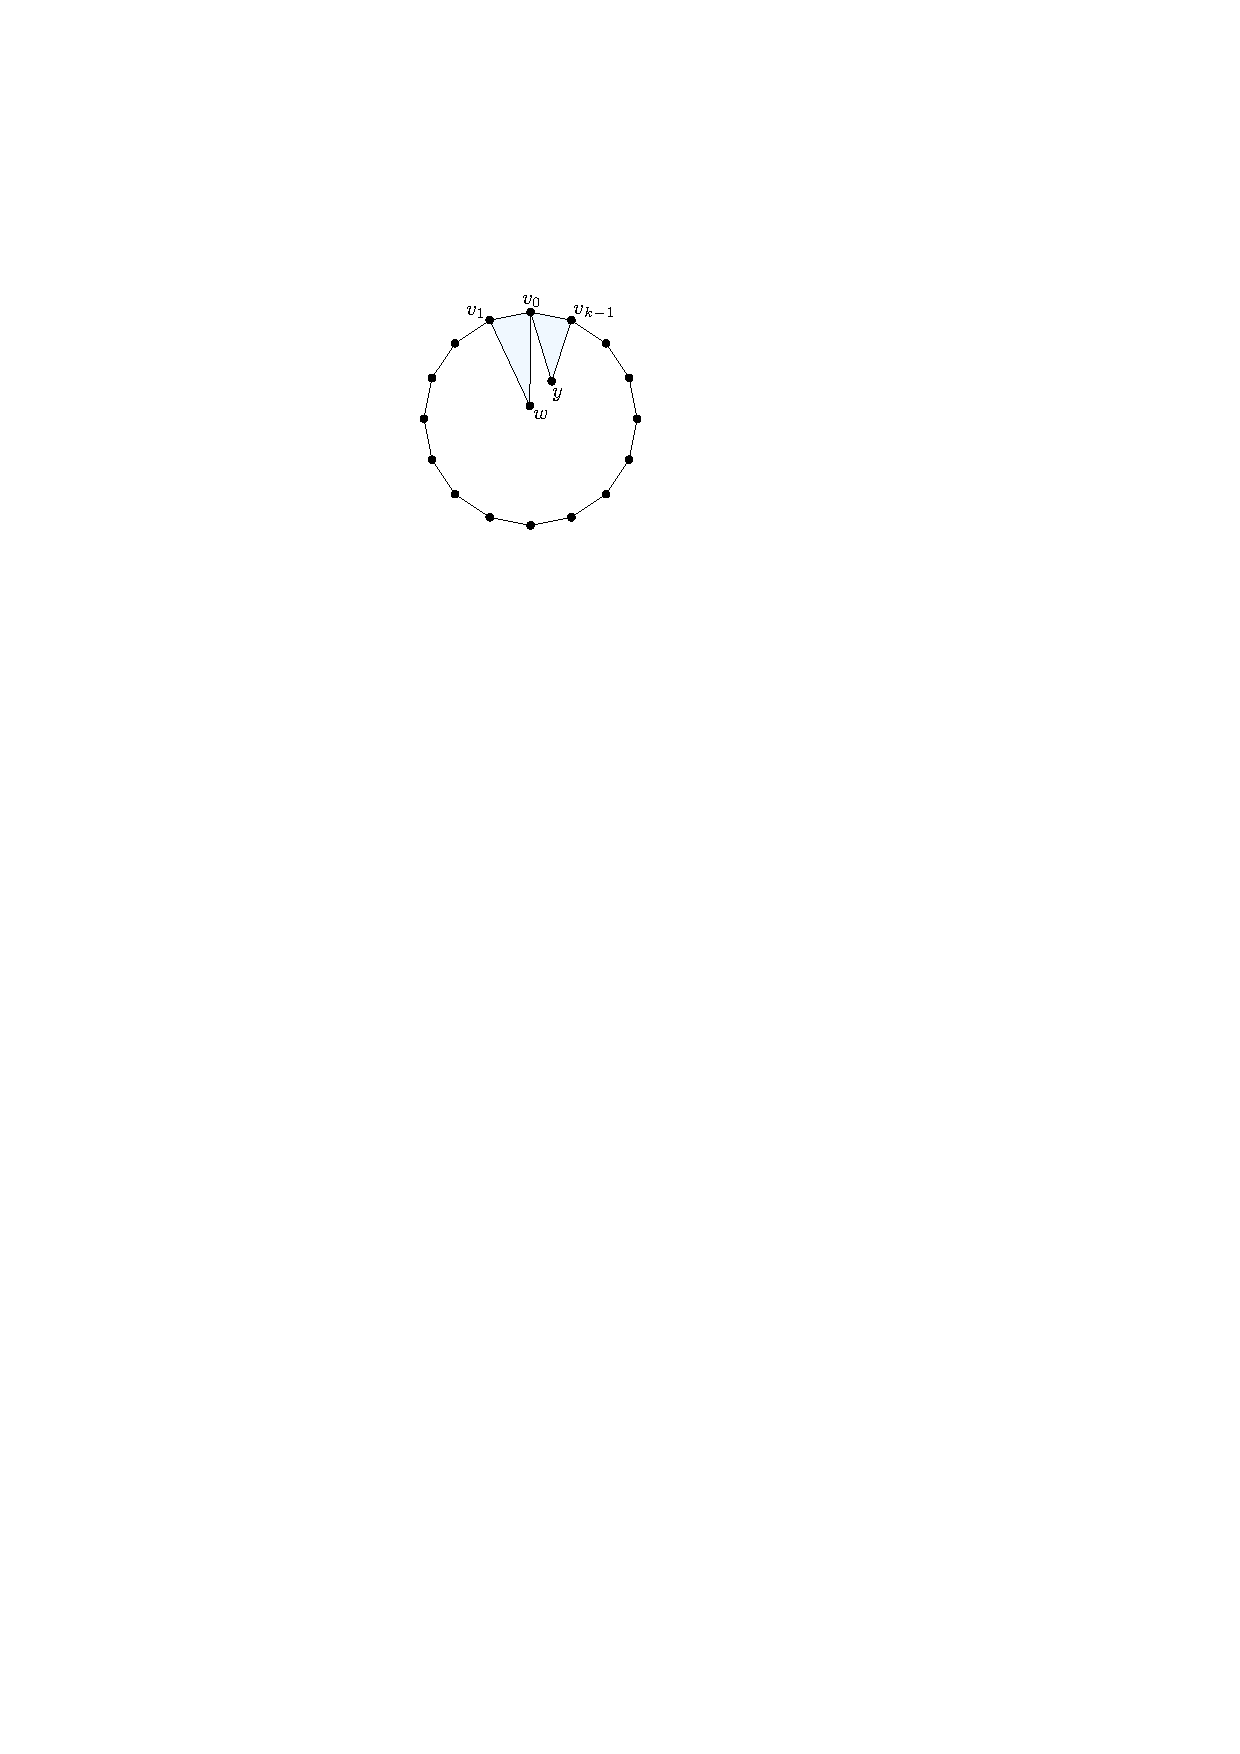
\includegraphics[page=1]{figs/really_good} &
        \includegraphics[page=2]{figs/really_good} &
        \includegraphics[page=3]{figs/really_good}
      \end{tabular}
    \end{center}
    \caption{The proof of \cref{really_good}}
    \label{really_good_fig}
  \end{figure}

  Let $v_0,\ldots,v_{k-1}$ be the cycle that bounds the inner face $f$ of $H[B(H)]$ that contains $w$ in its interior.  Since $H$ is a near-triangulation, $H$ contains triangles $v_0v_1x$ and $v_{k-1}v_0 y$ with $x$ and $y$ in the interior of or on the boundary of $f$.  Since $f$ is a face of $H[B(H)]$ each of $x$ and $y$ is in the interior of $f$.  At least one of $x$ or $y$ is equal to $w$, say $x$, since otherwise $\deg^+_H(v_0)\ge 3$.  Therefore $v_0v_1 w$ is an inner face of $H$.  Let $j\ge 1$ be the maximum integer such that $v_{a-1}v_{a}w$ is an inner face of $H$ for all $a\in\{1,\ldots,j\}$.  Note that $j<\ell-1$ since, otherwise, the component of $H-B(H)$ that contains $w$ contains only a single vertex, contradicting the fact that $\deg^+_{H-B(H)}(w)=2$.

  Since $H$ is a near-triangulation and $f$ is a face of $H$, $H$ has some face $v_j v_{j+1} z$ with $z$ in the interior of $f$.  By the definition of $j$, $z\neq w$.  Therefore, $N_H^+(v_j)\supseteq \{w,z\}$ and, since $\deg^+_H(v_j)\le 2$, $N_H^+(v_j))= \{w,z\}$.  Therefore $N^+_H(v_j)\subseteq N_H[w]$.

  All that remains is to show that $\deg^+_{H-v_0}(w)\ge 3$.  First, observe that $z$ is in $B(H-B(H))$, so $z$ does not contribute to $\deg^+_{H-B(H)}(w)$. We claim that $z$ is in $I(H-v_0)$, so $z$ does contribute to $\deg^+_{H-v_0}(w)$.  Indeed, the only other possibility is that $z$ is adjacent to $v_0$.  In this case, consider the cycle $C:=v_0,\ldots,v_j,z$.  This cycle has $w$ in its interior. The vertices of $N^+_{H-B(H)}(w)$ must be in the interior of $C$. For each $a\in\{1,\ldots,j\}$, $v_{a-1}v_a w$ is a face of $H$, so the cycle $D:=v_0,\ldots,v_j,w$ does not contain any vertices of $N^+_{H-B(H)}(w)$ in its interior.  Therefore, the vertices in $N^+_{H-B(H)}(w)$ must be in the interior of the cycle $\overline{D}:=v_0,w,v_j,z$.  Since $H$ is a near-triangulation, this implies that at least one of $v_0$ or $v_j$ is adjacent to some vertex in $I(H)\setminus\{w,z\}$. But this is not possible since it would imply that $\deg^+_H(v_0)\ge 3$ or $\deg^+_H(v_j)\ge 3$.  Therefore $v_0$ is not adjacent to $z$, so $z$ is in the interior of $H-v_0$ and $N^+_{H-v_0}(w)\supseteq N^+_{H-B(H)}(w)\uplus\{z\}$, so $\deg^+_H(w)\ge 3$.
\end{proof}

\begin{lem}\label{big_boundary}
  Let $H$ be a dom-minimal generalized near-triangulation with $\deg^+_H(v)\le 2$ for each $v\in B(H)$.  Then $|B(H)|\ge |B(H-B(H))|$.
\end{lem}

\begin{proof}
  Each vertex $w$ in $B(H-B(H))$ is adjacent to at least one vertex $v_0$ on the outer face of $H$.  The vertex $v_0$ has two neighbours $v_{-1}$ and $v_1$ on the outer face of $H$. Since $H$ is dom-minimal, it contains faces $v_0v_1x$ and $v_0v_{-1}y$ with $x$ and $y$ being inner vertices of $H$.  Then at least one of $x$ or $y$ must be $w$ since, otherwise, $\deg^+_H(v_0)\ge 3$ \pat{Explain}.   But then $w$ is adjacent to at least one of $v_{-1}$ or $v_1$.  Therefore $w$ is adjacent to at least two vertices in $B(H)$.  Therefore, each $w\in B(H-B(H))$ contributes at least $2$ to $\sum_{v\in B(H)}\deg^+_H(v)$, so $2|B(H)|\ge \sum_{v\in B(H)}\deg^+_H(v)\ge 2|B(H-H(B))|$, as required.
\end{proof}

We say that a generalized near-triangulation $H$ is \defin{$2$-critical} if $H-B(H)$ is critical and $\deg^+_H(v)\le 2$ for each $v\in B(H)$.  Observe that any critical graph is also $2$-critical.

\begin{lem}\label{two_critical_handler}
  Let $H$ be a $2$-critical dom-minimal generalized near-triangulation.  Then there exists $X\subseteq V(H)$ of size at most $2|B(H-B(H))|/3$ such that $I(H)\subseteq N_H[X]$.
\end{lem}

\begin{proof}
  Let $H_0$ be a graph obtained by triangulating the inner faces of $H[B(H-B(H))]$. Now $3$-colour $H_0$ and let $X$ be the smallest colour class.
  For each vertex $w\in X$, choose a vertex $v\in N_H(w)\cap B(H)$ and put $v$ in $X$.  The size of the resulting set $X$ is at most $2|X_0|\le 2|B(H-B(H))|/3$.
\end{proof}


\subsection{The Algorithm}

This gives variant of the $\textsc{SimpleGreedy}(G)$ that we call $\textsc{BestGreedy}(G)$.  Suppose we have already chosen $\Delta_0,\ldots,\Delta_{i-1}$ for some $i\ge 0$ and we now want to choose $\Delta_i$.  Let $X_i:=\bigcup_{j=0}^{i-1}\Delta_j$, let $G_i$ be a dom-preserving subgraph of $G-X_i$ that is dom-minimal, and let $v_i$ be a vertex in $B(G_i)$ that maximizes $\deg^+_{G_i}(v_i)$.  During iteration $i\ge 0$, there are now three cases to consider:
\begin{compactenum}
    \item If $\deg^+_{G_i}(v_i)\ge 3$ then we set $\Delta_i\gets\{v_i\}$.
    \item If there exists distinct $u,v\in B(G_i)$ and $w\in B(G_i-B(G_i))$ such that $\deg^+_{G_i}(v)=2$, $\deg^+_{G_i-v}(w)\ge 3$, and $N^+_{G_i}(u)\subseteq N_{G_i}(w)$ then set $\Delta_i:=\{v,w\}$.
    \item Otherwise, $G_i$ is $2$-critical and $i+1=r$.  By \cref{two_critical_handler}, there exists $\Delta_{r-1}\subseteq V(G_i)$ of size at most $|B(G_i-B(G_i))|/3 + |I(G_i[I(G_i)])|$ that dominates $I(G_i)$.
\end{compactenum}

\begin{thm}\label{best_greedy}
  When applied to an $n$-vertex triangulation $G$,  $\textsc{BestGreedy}(G)$ produces a connected dominating set $X_r$ of size at most $7n/15\pm O(1)$.
\end{thm}

\begin{proof}
  For each integer $t\ge 3$, let $x_t$ be the number of times $\textsc{BetterGreedy}(G)$ falls into case $1$ and chooses $v_i$ such that $\deg^+_{G_i}(v_i)=t$.  Let $z$ be the number of times $\textsc{BetterGreedy}(G)$ falls into Case~2.  Let
  \[
     D:=|D_{r-1}| = 3 + \sum_{t\ge 3}tx_t + 5z \enspace .
  \]
  Let $I:=|I(G_{r-1})$, let $B:=|B(G_{r-1})|$, let $Q:=|B(G_{r-1}-B(G_{r-1}))|$ and let $R:=|I(G_{r-1}-B(G_{r-1}))|$.  Then, by \cref{big_boundary} and \cref{base_case}
  \begin{equation}
    Q \ge R \ge 3S \enspace . \label{best2}
  \end{equation}
  By definition $r-1 = \sum_{t\ge 3}x_t+z$.
  As in the proofs of \cref{simple_greedy} and \cref{better_greedy}, $D+|I(G_i)|=D+R+S=n$, so we get the constraint:
  \begin{equation}
    n = D+R+S \ge \sum_{t\ge 3} tx_t + 5z + R + S \label{best3}
  \end{equation}
  and
  \begin{equation}
    n = D+R+S \ge r-1 + Q + R + S \enspace . \label{best4}
  \end{equation}
  Finally, the size $Q$ of the boundary $B(G_{r-1})$ is at most
  \begin{equation}
    Q \le 3 + \sum_{t\ge 3}(t-1)x_t + 2z \label{best5}
  \end{equation}
  By \cref{two_critical_handler}, the size of $\Delta_{r-1}$ is at most $R/3+ S$, so the total size of the final set $X$ is at most
  \begin{equation}
    r-1 + R/3 + S \enspace .  \label{best_objective}
  \end{equation}
  As in the proof of \cref{better_greedy}, we can eliminate the variables $x_t$ for $t\ge 4$:
  \begin{clm}
    In any assignment of non-negative values to $Q, R, S$, $z$, and $x_3,x_4\ldots$ that maximizes \cref{best_objective} subject to \cref{best2,best3,best4,best5}, $x_t=0$ for all $t\ge 4$.
  \end{clm}
  \begin{clmproof}
     If $x_t = c >0$ for some $t\ge 4$, then we can set $x_t\gets 0$, $x_3\gets x_3+tc/3$, \ldots \pat{Finish this....}
  \end{clmproof}
  \begin{clm}
    In any assignment of non-negative values to $Q, R, S$, $z$, and $x_3,x_4\ldots$ that maximizes \cref{best_objective} subject to \cref{best2,best3,best4,best5}, $z=0$.
  \end{clm}
  \begin{clmproof}
    If $z = c >0$  then we can set $z\gets 0$, $x_3\gets x_3+5c/3$, $Q\gets Q+10c/3-2c=Q+4c/3$, $R\gets 10c/3-2c=Q+4c/3$, and $S\gets 10c/9-2c/3=S+4c/9$. Then the objective function \cref{best_objective} increases by $(5/3+4/3+4/9)c >0$.  \Cref{best2} is still satisfied because the quantities $Q$, $R$, and $3S$ change by exactly the same amount.  \Cref{best3} is still satisfied because the right hand side decreases by $(5-4/3+4/3)c=7c/3$. \Cref{best4} still holds because the right hand side decreases by $4c/3 + 4c/3 +4c/9 - 5c/3>0$  \Cref{best5} still holds because the left hand side decreases by $4c/3$ and the right hand side increases by $10c/3 - 2c=4c/3$.

  \end{clmproof}
  Therefore, \cref{best2,best3,best4,best5} are inequalities in four non-negative variables $x_3$, $Q$, $R$ and $S$.  Maximizing \cref{best_objective} subject to these constraints is an easy linear programming exercise and the maximum is achieved when $x_3=(n-6)/5$, $Q=R=(2n+3)/5$, $S=0$, giving a final bound of $|X|\le r-1+R/3\le (7n-12)/15$.
\end{proof}


% \section{Moonshot}
%
% We say that a near-triangulation $H$ is \defin{dom-minimal} if
% \begin{compactenum}[({DM}1)]
%     \item each vertex $v\in B(H)$ has $\deg^+_H(v)\ge 1$; \label[dm]{minimum_degree}
%     \item if there exists edges $uv$ and $vw$ on the outer face of $H$ and  $\deg^+_H(v)\ge 1$ then $uw$ is an edge of $H$; and \label[dm]{one_vertex}
%     \item each edge $vw$ on the boundary of the outer face of $H$ is on the boundary an inner face $vxw$ of $H$ for some $x\in I(H)$. \label[dm]{bad_edge}
% \end{compactenum}
% We say that a generalized near-triangulation $H$ is \defin{dom-minimal} if each of its biconnected components are dom-minimal.
%
% \begin{obs}\label{bridgeless}
%     Any dom-minimal generalized near-triangulation $H$ is bridgeless.
% \end{obs}
%
% \begin{proof}
%    If $vw$ is a bridge in $H$ then both $v$ and $w$ are in $B(H)$.  Since $vw$ is a bridge in $H$, there is no path $vxw$ in $H$ and therefore no inner face $vwx$ in $H$. Thus $H$ does not satisfy \cref{bad_edge}.
% \end{proof}
%
% \begin{lem}\label{chord_incident}
%   let $H$ be a (biconnected) dom-minimal non-critical near-triangulation and let $v_0$ be a vertex in $B(H)$ with $|N_H(v_0)\cap B(H)|\ge 3$.  Then $\deg^+_H(v_0)\ge 2$.  In other words, if $v_0$ is incident to a chord of the outerplane graph $H[B(H)]$, then $v_0$ is incident to at least $2$ inner vertices of $H$.
% \end{lem}
%
% \begin{figure}[htbp]
%   \begin{center}
%     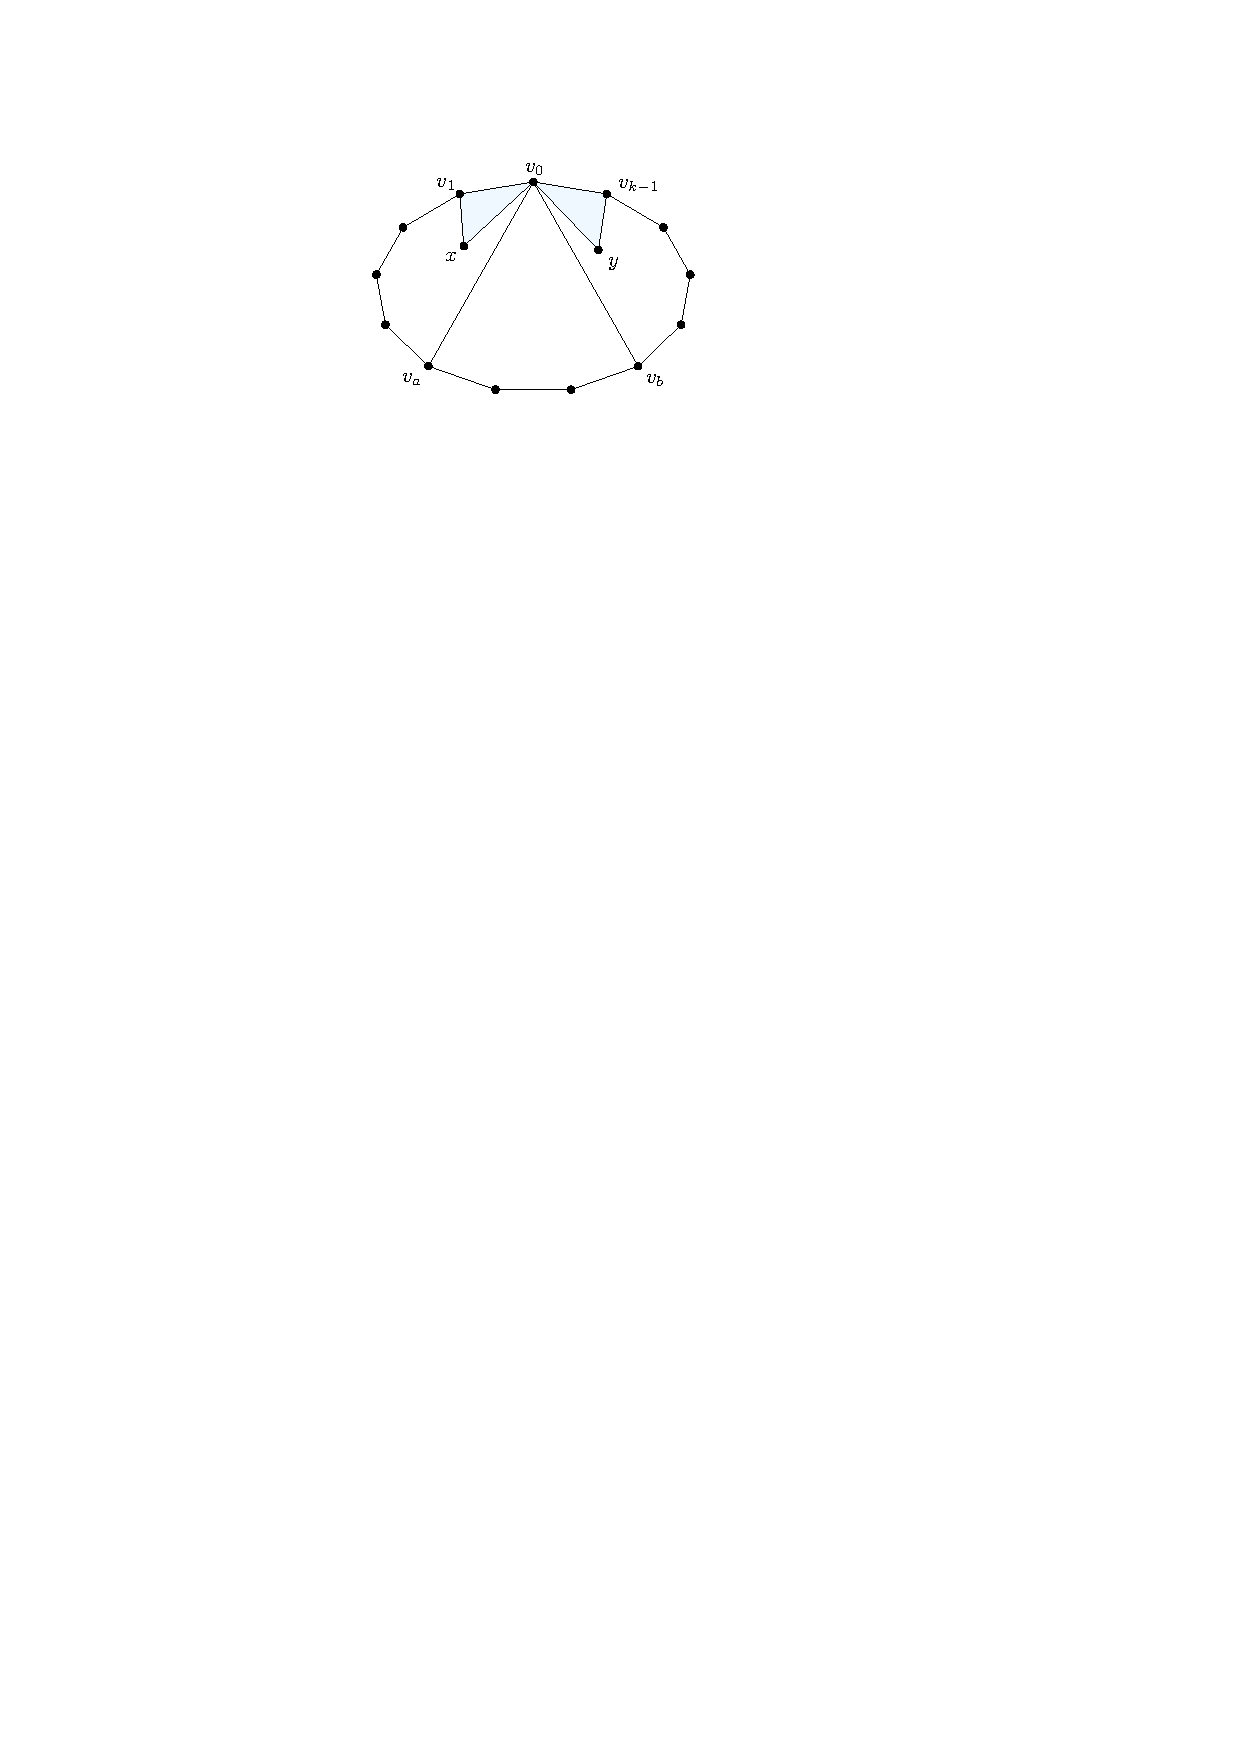
\includegraphics{figs/chord_incident}
%   \end{center}
%   \caption{The proof of \cref{chord_incident}}
%   \label{chord_incident_fig}
% \end{figure}
% \begin{proof}
%   Refer to \cref{chord_incident_fig}
%   Since $H$ is a near-triangulation its outer face is bounded by a cycle $v_0,\ldots,v_{k-1}$.  Let $a:=\min\{i\in\{2,\ldots,k-2\}:v_0v_i\in E(H)\}$ and $b:=\max\{i\in\{2,\ldots,k-2\}:v_0v_i\in E(H)\}$. (Possibly $a=b$, but both $a$ and $b$ are well-defined since $|N^+_H(v_0)|\ge 3$.)   Since $H$ is dom-minimal, the edge $v_0v_1$ is on the boundary of an inner face $v_0v_1x$ of $H$ where $x$ is an inner vertex of $H$.  Since $H$ is dom-minimal, the edge $v_{k-1}v_0$ is on the boundary of an inner face $v_{k-1}v_0y$ of $H$ where $y$ is an inner vertex of $H$.  Then $x$ is in the interior of the face of $H[B(H)]$ bounded by the cycle $v_0,v_1,\ldots,v_a$ and $y$ is in the interior of the face of $H[B(H)]$ bounded by the cycle $v_0,v_b,\ldots,v_{k-1}$.  Therefore, $x\neq y$ and $N^+_H(v_0)\supseteq\{x,y\}$ so $\deg^+_H(v_0)\ge 2$.
% \end{proof}
%
%
%
% Let $K_5^-$ be the complete graph on five vertices with one edge removed.
%
% \begin{lem}
%   Let $H$ be a near-triangulation with $\deg^+_H(z)\le 2$ for all $z\in B(H)$. If $\deg^+_H(v)=1$ for some $v\in B(H)$, then $H$ is isomorphic to $K_4$ or $K_5^-$.
% \end{lem}
%
% \begin{proof}
%   Since $H$ is dom-minimal each vertex in $B(H)$ has inner-degree at least $1$, by \cref{minimum_degree}.  Therefore the outer face of $H$ is a cycle with at least three vertices.  Let $u$ and $w$ be the two neighbours of $v$ on the outer face.  Since $H$ is dom-minimal, $H$ contains an inner face $vxu$ with $x\in I(H)$, by \cref{bad_edge}.  Since $H$ is dom-minimal, $H$ contains an inner face $wyv$ with $y\in I(H)$.  Since $\deg^+_H(v)=1$, $x=y$.  Since $H$ is dom-minimal $uw$ is an edge of $H$, by \cref{one_vertex}.  Therefore $uvx
% \end{proof}
%
% A subgraph $H'$ of a generalized near-triangulation $H$ is \defin{dom-preserving} if
% % every outer-domatic set $X\subseteq V(H')$ of $H'$ is an outer-domatic set of $H$.
%
% \begin{compactenum}[({DP}1)]
%   \item $B(H')\subseteq B(H)$; \label[dp]{smaller_boundary}
%   \item $N^+_{H'}(v)=N^+_H(v)$ for all $v\in B(H')$; \label[dp]{interior_preserving}
%   \item $I(H')=I(H)$; and \label[dp]{inner_neighbourhood_preserving}
%   \item $N_{H'}(v)=N_H(v)\cap V(H')$ for all $v\in I(H)$. \label[dp]{outer_neighbour_preserving}
% \end{compactenum}
%
% \begin{obs}
%   Let $H$ be a generalized near-triangulation, let $H'$ be a dom-preserving subgraph of $H$, and let $\Delta$ be a subset of $V(H')$ that dominates $I(H')$ in $H'$.  Then $\Delta$ dominates $I(H)$ in $H$.
% \end{obs}
%
% % \begin{proof}
% %   Each vertex $v\in I(H')$ is adjacent to some vertex $w\in \Delta$.  Since $N_{H'}(v)=N_H(v)$, $w\in\Delta\cap V(H')$, so $v$ is dominated by $\Delta\cap V(H')$.  Since this is true for each $v\in I(H)=I(H')$, $\Delta\cap V(H')$ dominates $I(H)$.
% % \end{proof}
%
% \begin{lem}\label{dom_minimal}
%   For any generalized near-triangulation $H$, there exists a dom-preserving subgraph $H'$ of $H$ that is dom-minimal.
% \end{lem}
%
% \begin{proof}
%   The proof is by induction on $|V(H)|+|E(H)|$.  If $H$ is already dom-minimal, then setting $H'=H$ satisfies the requirements of the lemma, so assume that $H$ is not dom-minimal.  It is straightforward to verify that the dom-preserving subgraph relationship is transitive, so if $H$ has a dom-preserving subgraph $H^*$ and $H^*$ has a dom-preserving subgraph $H'$ then $H'$ is a dom-preserving subgraph of $H$.  Therefore, it is sufficient to show the existence of a dom-preserving subgraph $H^*$ of $H$ with fewer edges or fewer vertices than $H$. Then the inductive hypothesis provides the desired dom-minimal dom-preserving subgraph $H'$ of $H$.
%
%   If $H$ contains a vertex $v\in B(H)$ with $\deg^+_H(v)=0$ then $H-v$ is a dom-preserving subgraph of $H$ with fewer vertices than $H$.  We now assume that $\deg^+_H(v)\ge 1$ for all $v\in B(H)$.  Since $H$ is not dom-minimal then $H$ contains a biconnected component $C$ that is not dom-minimal.
%   \begin{compactenum}
%     \item If there exists an edge $vw$ on the outer face of $C$ that is not incident to any inner face $vxw$ with $x\in I(C)$ then $B(H-vw)=B(H)$ and $I(H-vw)=I(H)$, and $H-vw$ is a is dom-preserving subgraph of $H$ that has fewer edges than $H$.
%
%     \item If there exists a vertex $v\in B(C)$ with $\deg^+_C(v)=0$ then $v$ is incident to an edge $vw$ that is on the outer face of $C$ and on the outer face of $H$. Since $\deg^+_C(v)=0$, $vw$ is not incident to any inner face $vwx$ with $x\in I(C)$ and we can proceed as in the previous case. \qedhere
%   \end{compactenum}
% \end{proof}
%


\bibliographystyle{plainurl}
\bibliography{main}

\end{document}
